\chapter{Генетический алгоритм} \label{ParticleSwarmOptimisation}
%\addcontentsline{toc}{chapter}{Метод роения частиц}    % Добавляем его в оглавление, если нет нумерации
\noindent
\emph{Генетический алгоритм} (\emph{Genetic Algorithm}, GA) является одним из самых популярных типов эволюционных алгоритмов, которые — как можно понять из их названия, — используют теорию эволюции, в частности теорию Дарвина, в решении той или иной оптимизационной задачи. Суть алгортима заключается в поиске наилучшего решения по принципу естественного отбора: случайным образом создается поколение, в ходе эволюции которого происходит скрещевание генов --- таким образом, появлется новое поколение (старые особи создают потомков) --- и их мутация.

\section{Алгоритм}
\noindent
Традиционно в качестве решения генетический алгоритм использует бинарное кодирование (binary encoding). Однако в данной работе будет проиллюстрирован метод реального кодирования (real value encoding), то есть решение будет представляться в вещественных числах.

Рассмотрим задачу нахождения глобального минимума функции~$F \colon \mathbb{R}^n \to \mathbb{R}$:
\[
	\mathop{\mathrm{argmin}}_{x \in \mathbb{R}^n}f(x),
\]
где каждая особь кодируется вектором $x = (x_1, ..., x_n)$, называемым хромосомой, компоненты которого являются генами.

\begin{figure}[!h]
\centering
\tikzset{every picture/.style={line width=0.75pt}} %set default line width to 0.75pt

\begin{tikzpicture}[x=0.75pt,y=0.75pt,yscale=-1,xscale=1]
%uncomment if require: \path (0,739); %set diagram left start at 0, and has height of 739

%Shape: Rectangle [id:dp8612057014709158]
\draw   (80,71) -- (110.5,71) -- (110.5,100) -- (80,100) -- cycle ;
%Shape: Rectangle [id:dp9416262412972431]
\draw   (110.5,71) -- (141,71) -- (141,100) -- (110.5,100) -- cycle ;
%Shape: Rectangle [id:dp9259667143051737]
\draw   (141,71) -- (171.5,71) -- (171.5,100) -- (141,100) -- cycle ;
%Shape: Rectangle [id:dp4285081026342692]
\draw   (171.5,71) -- (202,71) -- (202,100) -- (171.5,100) -- cycle ;
%Shape: Rectangle [id:dp6066867188861804]
\draw   (202,71) -- (232.5,71) -- (232.5,100) -- (202,100) -- cycle ;
%Curve Lines [id:da8858061911822572]
\draw    (232.5,71) .. controls (289.5,72) and (230.5,126) .. (308.5,126) ;
%Straight Lines [id:da05811670243584288]
\draw    (158.5,45) -- (158.5,68) ;
\draw [shift={(158.5,70)}, rotate = 270] [color={rgb, 255:red, 0; green, 0; blue, 0 }  ][line width=0.75]    (10.93,-3.29) .. controls (6.95,-1.4) and (3.31,-0.3) .. (0,0) .. controls (3.31,0.3) and (6.95,1.4) .. (10.93,3.29)   ;
%Shape: Rectangle [id:dp4349277402828884]
\draw   (81,151) -- (111.5,151) -- (111.5,180) -- (81,180) -- cycle ;
%Shape: Rectangle [id:dp24027028194138378]
\draw   (111.5,151) -- (142,151) -- (142,180) -- (111.5,180) -- cycle ;
%Shape: Rectangle [id:dp0500263413916362]
\draw   (142,151) -- (172.5,151) -- (172.5,180) -- (142,180) -- cycle ;
%Shape: Rectangle [id:dp8133255101181311]
\draw   (172.5,151) -- (203,151) -- (203,180) -- (172.5,180) -- cycle ;
%Shape: Rectangle [id:dp367355050028054]
\draw   (203,151) -- (233.5,151) -- (233.5,180) -- (203,180) -- cycle ;
%Curve Lines [id:da7627402544422663]
\draw    (233.5,180) .. controls (290.5,181) and (230.5,126) .. (308.5,126) ;
%Shape: Circle [id:dp7594178378532763]
\draw   (113.75,165.5) .. controls (113.75,158.32) and (119.57,152.5) .. (126.75,152.5) .. controls (133.93,152.5) and (139.75,158.32) .. (139.75,165.5) .. controls (139.75,172.68) and (133.93,178.5) .. (126.75,178.5) .. controls (119.57,178.5) and (113.75,172.68) .. (113.75,165.5) -- cycle ;
%Straight Lines [id:da7888876982561981]
\draw    (161.5,202) -- (131.49,175.33) ;
\draw [shift={(130,174)}, rotate = 401.63] [color={rgb, 255:red, 0; green, 0; blue, 0 }  ][line width=0.75]    (10.93,-3.29) .. controls (6.95,-1.4) and (3.31,-0.3) .. (0,0) .. controls (3.31,0.3) and (6.95,1.4) .. (10.93,3.29)   ;

% Text Node
\draw (80,122) node [anchor=north west][inner sep=0.75pt]   [align=left] {..............................};
% Text Node
\draw (311,120) node [anchor=north west][inner sep=0.75pt]  [font=\small] [align=left] {Популяция};
% Text Node
\draw (123,30) node [anchor=north west][inner sep=0.75pt]  [font=\small] [align=left] {Хромосома};
% Text Node
\draw (85,78) node [anchor=north west][inner sep=0.75pt]  [font=\small] [align=left] {$\displaystyle x_{11}$};
% Text Node
\draw (146,78) node [anchor=north west][inner sep=0.75pt]  [font=\small] [align=left] {$\displaystyle x_{13}$};
% Text Node
\draw (207,78) node [anchor=north west][inner sep=0.75pt]  [font=\small] [align=left] {$\displaystyle x_{1n}$};
% Text Node
\draw (115.5,78) node [anchor=north west][inner sep=0.75pt]  [font=\small] [align=left] {$\displaystyle x_{12}$};
% Text Node
\draw (179,82) node [anchor=north west][inner sep=0.75pt]   [align=left] {...};
% Text Node
\draw (86,158) node [anchor=north west][inner sep=0.75pt]  [font=\small] [align=left] {$\displaystyle x_{\ell 1}$};
% Text Node
\draw (147,158) node [anchor=north west][inner sep=0.75pt]  [font=\small] [align=left] {$\displaystyle x_{\ell 3}$};
% Text Node
\draw (208,158) node [anchor=north west][inner sep=0.75pt]  [font=\small] [align=left] {$\displaystyle x_{\ell n}$};
% Text Node
\draw (116.5,158) node [anchor=north west][inner sep=0.75pt]  [font=\small] [align=left] {$\displaystyle x_{\ell 2}$};
% Text Node
\draw (180,162) node [anchor=north west][inner sep=0.75pt]   [align=left] {...};
% Text Node
\draw (163.5,205) node [anchor=north west][inner sep=0.75pt]  [font=\small] [align=left] {Ген};
\end{tikzpicture}
\caption{}
\end{figure}

Пусть у нашего поколения, или популяции, $P$ есть $\ell$ особей. Тогда поколение в момент времени $t$ примет следующий вид:
\[
	P_t = \{x_{i,t}\}_{i=1}^\ell,
\]
где у кажой хромосомы имеется $n$ генов: $x_{i, t} = (x_{i1,t}, ..., x_{in, t})$

\begin{figure}[!h]
	\centering


	\tikzset{every picture/.style={line width=0.75pt}} %set default line width to 0.75pt

	\begin{tikzpicture}[x=0.75pt,y=0.75pt,yscale=-1,xscale=1]
	%uncomment if require: \path (0,739); %set diagram left start at 0, and has height of 739


	%Rounded Rect [id:dp6834144691063508]
	\draw  [color={rgb, 255:red, 128; green, 128; blue, 128 }  ,draw opacity=1 ][fill={rgb, 255:red, 155; green, 155; blue, 155 }  ,fill opacity=0.06 ] (240.5,57) .. controls (240.5,48.16) and (247.66,41) .. (256.5,41) -- (474.5,41) .. controls (483.34,41) and (490.5,48.16) .. (490.5,57) -- (490.5,105) .. controls (490.5,113.84) and (483.34,121) .. (474.5,121) -- (256.5,121) .. controls (247.66,121) and (240.5,113.84) .. (240.5,105) -- cycle ;
	%Rounded Rect [id:dp6349764616806755]
	\draw   (400.5,316) .. controls (400.5,307.16) and (407.66,300) .. (416.5,300) -- (634.5,300) .. controls (643.34,300) and (650.5,307.16) .. (650.5,316) -- (650.5,364) .. controls (650.5,372.84) and (643.34,380) .. (634.5,380) -- (416.5,380) .. controls (407.66,380) and (400.5,372.84) .. (400.5,364) -- cycle ;
	%Rounded Rect [id:dp3411925739284387]
	\draw   (79.5,316) .. controls (79.5,307.16) and (86.66,300) .. (95.5,300) -- (313.5,300) .. controls (322.34,300) and (329.5,307.16) .. (329.5,316) -- (329.5,364) .. controls (329.5,372.84) and (322.34,380) .. (313.5,380) -- (95.5,380) .. controls (86.66,380) and (79.5,372.84) .. (79.5,364) -- cycle ;
	%Rounded Rect [id:dp15356651288080547]
	\draw  [color={rgb, 255:red, 128; green, 128; blue, 128 }  ,draw opacity=1 ][fill={rgb, 255:red, 155; green, 155; blue, 155 }  ,fill opacity=0.06 ] (241.5,187) .. controls (241.5,178.16) and (248.66,171) .. (257.5,171) -- (475.5,171) .. controls (484.34,171) and (491.5,178.16) .. (491.5,187) -- (491.5,235) .. controls (491.5,243.84) and (484.34,251) .. (475.5,251) -- (257.5,251) .. controls (248.66,251) and (241.5,243.84) .. (241.5,235) -- cycle ;
	%Rounded Rect [id:dp13735168020488797]
	\draw  [color={rgb, 255:red, 128; green, 128; blue, 128 }  ,draw opacity=1 ][fill={rgb, 255:red, 155; green, 155; blue, 155 }  ,fill opacity=0.06 ] (400.5,316) .. controls (400.5,307.16) and (407.66,300) .. (416.5,300) -- (634.5,300) .. controls (643.34,300) and (650.5,307.16) .. (650.5,316) -- (650.5,364) .. controls (650.5,372.84) and (643.34,380) .. (634.5,380) -- (416.5,380) .. controls (407.66,380) and (400.5,372.84) .. (400.5,364) -- cycle ;
	%Rounded Rect [id:dp18159494190384895]
	\draw  [color={rgb, 255:red, 128; green, 128; blue, 128 }  ,draw opacity=1 ][fill={rgb, 255:red, 155; green, 155; blue, 155 }  ,fill opacity=0.06 ] (240.5,446) .. controls (240.5,437.16) and (247.66,430) .. (256.5,430) -- (474.5,430) .. controls (483.34,430) and (490.5,437.16) .. (490.5,446) -- (490.5,494) .. controls (490.5,502.84) and (483.34,510) .. (474.5,510) -- (256.5,510) .. controls (247.66,510) and (240.5,502.84) .. (240.5,494) -- cycle ;
	%Rounded Rect [id:dp23454056652855249]
	\draw  [color={rgb, 255:red, 128; green, 128; blue, 128 }  ,draw opacity=1 ][fill={rgb, 255:red, 155; green, 155; blue, 155 }  ,fill opacity=0.06 ] (79.5,316) .. controls (79.5,307.16) and (86.66,300) .. (95.5,300) -- (313.5,300) .. controls (322.34,300) and (329.5,307.16) .. (329.5,316) -- (329.5,364) .. controls (329.5,372.84) and (322.34,380) .. (313.5,380) -- (95.5,380) .. controls (86.66,380) and (79.5,372.84) .. (79.5,364) -- cycle ;
	%Rounded Rect [id:dp04080350160967616]
	\draw  [color={rgb, 255:red, 128; green, 128; blue, 128 }  ,draw opacity=1 ][fill={rgb, 255:red, 155; green, 155; blue, 155 }  ,fill opacity=0.06 ] (140.38,566.82) .. controls (140.38,563.61) and (142.99,561) .. (146.2,561) -- (324.56,561) .. controls (327.77,561) and (330.38,563.61) .. (330.38,566.82) -- (330.38,584.28) .. controls (330.38,587.49) and (327.77,590.1) .. (324.56,590.1) -- (146.2,590.1) .. controls (142.99,590.1) and (140.38,587.49) .. (140.38,584.28) -- cycle ;
	%Rounded Rect [id:dp20329352519352284]
	\draw  [color={rgb, 255:red, 128; green, 128; blue, 128 }  ,draw opacity=1 ][fill={rgb, 255:red, 155; green, 155; blue, 155 }  ,fill opacity=0.06 ] (400.38,566.82) .. controls (400.38,563.61) and (402.99,561) .. (406.2,561) -- (584.56,561) .. controls (587.77,561) and (590.38,563.61) .. (590.38,566.82) -- (590.38,584.28) .. controls (590.38,587.49) and (587.77,590.1) .. (584.56,590.1) -- (406.2,590.1) .. controls (402.99,590.1) and (400.38,587.49) .. (400.38,584.28) -- cycle ;
	%Straight Lines [id:da8542759790833123]
	\draw [line width=0.75]    (100.5,381) -- (100.01,458) ;
	\draw [shift={(100,460)}, rotate = 270.36] [color={rgb, 255:red, 0; green, 0; blue, 0 }  ][line width=0.75]    (15.3,-6.86) .. controls (9.73,-3.22) and (4.63,-0.93) .. (0,0) .. controls (4.63,0.93) and (9.73,3.22) .. (15.3,6.86)   ;
	%Curve Lines [id:da3464775501690811]
	\draw    (492,210) .. controls (540.51,210) and (529.23,248.22) .. (529.97,298.47) ;
	\draw [shift={(530,300)}, rotate = 268.88] [color={rgb, 255:red, 0; green, 0; blue, 0 }  ][line width=0.75]    (10.93,-4.9) .. controls (6.95,-2.3) and (3.31,-0.67) .. (0,0) .. controls (3.31,0.67) and (6.95,2.3) .. (10.93,4.9)   ;
	%Curve Lines [id:da05243098101616073]
	\draw    (530,381) .. controls (530,430.5) and (537.84,469.22) .. (491.42,469.99) ;
	\draw [shift={(490,470)}, rotate = 360] [color={rgb, 255:red, 0; green, 0; blue, 0 }  ][line width=0.75]    (10.93,-4.9) .. controls (6.95,-2.3) and (3.31,-0.67) .. (0,0) .. controls (3.31,0.67) and (6.95,2.3) .. (10.93,4.9)   ;
	%Curve Lines [id:da3734166178553002]
	\draw    (239,470) .. controls (190.49,470) and (199.81,431.78) .. (200,382.5) ;
	\draw [shift={(200,381)}, rotate = 450] [color={rgb, 255:red, 0; green, 0; blue, 0 }  ][line width=0.75]    (10.93,-4.9) .. controls (6.95,-2.3) and (3.31,-0.67) .. (0,0) .. controls (3.31,0.67) and (6.95,2.3) .. (10.93,4.9)   ;
	%Curve Lines [id:da337716542230607]
	\draw    (199,299) .. controls (199.99,251.48) and (190.2,210.82) .. (239.49,210.01) ;
	\draw [shift={(241,210)}, rotate = 180] [color={rgb, 255:red, 0; green, 0; blue, 0 }  ][line width=0.75]    (10.93,-4.9) .. controls (6.95,-2.3) and (3.31,-0.67) .. (0,0) .. controls (3.31,0.67) and (6.95,2.3) .. (10.93,4.9)   ;
	%Straight Lines [id:da3596375703194834]
	\draw  [dash pattern={on 0.84pt off 2.51pt}]  (359,511) -- (240,557) ;
	%Straight Lines [id:da6375981239192003]
	\draw  [dash pattern={on 0.84pt off 2.51pt}]  (359,511) -- (498,561) ;
	%Straight Lines [id:da4776300035987695]
	\draw [line width=0.75]    (364.5,121) -- (364.98,170) ;
	\draw [shift={(365,172)}, rotate = 269.44] [color={rgb, 255:red, 0; green, 0; blue, 0 }  ][line width=0.75]    (15.3,-6.86) .. controls (9.73,-3.22) and (4.63,-0.93) .. (0,0) .. controls (4.63,0.93) and (9.73,3.22) .. (15.3,6.86)   ;

	% Text Node
	\draw (300,180) node [anchor=north west][inner sep=0.75pt]  [font=\small,rotate=-359.78] [align=left] {\begin{minipage}[lt]{86.87pt}\setlength\topsep{0pt}
	\begin{center}
	{\fontfamily{helvet}\selectfont Расчет функции }\\{\fontfamily{helvet}\selectfont приспособленности}
	\end{center}

	\end{minipage}};
	% Text Node
	\draw (300,50) node [anchor=north west][inner sep=0.75pt]  [font=\small] [align=left] {\begin{minipage}[lt]{93.95696000000001pt}\setlength\topsep{0pt}
	\begin{center}
	{\fontfamily{helvet}\selectfont Создание поколения }\\t = 0
	\end{center}

	\end{minipage}};
	% Text Node
	\draw (500,331.8) node [anchor=north west][inner sep=0.75pt]  [font=\small] [align=left] {Отбор};
	% Text Node
	\draw (190,567.8) node [anchor=north west][inner sep=0.75pt]  [font=\small] [align=left] {Скрещивание};
	% Text Node
	\draw (470,567.76) node [anchor=north west][inner sep=0.75pt]  [font=\small] [align=left] {Мутация};
	% Text Node
	\draw (90,333.8) node [anchor=north west][inner sep=0.75pt]  [font=\small] [align=left] {Критерий останова выполнен?};
	% Text Node
	\draw (260,440) node [anchor=north west][inner sep=0.75pt]  [font=\small] [align=left] {\begin{minipage}[lt]{144.88216000000003pt}\setlength\topsep{0pt}
	\begin{center}
	Формирование нового поколения\\t = t + 1
	\end{center}

	\end{minipage}};
	% Text Node
	\draw (165,246.8) node [anchor=north west][inner sep=0.75pt]  [font=\small] [align=left] {Нет};
	% Text Node
	\draw (109.5,404.8) node [anchor=north west][inner sep=0.75pt]  [font=\small] [align=left] {Да};
	% Text Node
	\draw (82.5,463.8) node [anchor=north west][inner sep=0.75pt]  [font=\small] [align=left] {Выход};
	\end{tikzpicture}
	\caption{ --- Генетический алгоритм.}
	\label{img:GA}
\end{figure}

\noindent
Теперь рассмотрим сам алгоритм, который также представлен на рисунке \ref{img:GA}:

\begin{enumerate}
	\item Генерируем первое поколение особей случайным образом:
	\[
		P_0 = \{x_{1, 0}, ..., x_{\ell, 0} \ | \ (x_{i1, 0}, ..., x_{in, 0}) \in D, \  x_{ij, 0} \sim U(a, b)\},
	\]
	где $D = \{(x_1, ..., x_n) \in \mathbb{R}^n \ | \  a < x_i < b,\ \ a,\ b \in \mathbb{R} \} $~--- заданная область оптимизации (гиперкуб или гиперпрямоугольник).

	\item Оцениваем приспособленность (fitness) текущего поколения.

	Сначала вычисляем значения целевой функции  для каждой особи:
	\[
		F_t = \{f(x_{i,t})\}_{i=1}^\ell
	\]
	Затем используем такое преобразование $\sigma$, что все комоненты $F_t$ будут лежать на отрезке $[0, 1]$:
	\begin{equation}
		\label{eq:normalization}
		\sigma(z) = \dfrac{z - F^{worst}}{F^{best} - F^{worst}},
	\end{equation}
	где $F^{best}$, $F^{worst}$~--- лучшее и худшее значения целевой функции в текущем поколении соответственно.

	Таким образом, получим значения приспособленности особей:
	\[
	F'_t = \{\sigma(f(x_{i, t}))\}_{i=1}^\ell
	\]

	\item  Отбирем $k$ наиболее преспособленных особей для дальнейшего размножения.

	Будем считать, что особь $x'$ более приспособлена, чем особь $x''$, если
	\[
		\sigma(f(x')) > \sigma(f(x''))
	\]
	Ранжируем особи в текущей популяции по значениям их приспособленности в порядке убывания, то есть от самых приспособленных к самым неприспособленным:
	\[
		\sigma(f(x^{(1)}_t)) \geq ... \geq \sigma(f(x^{(k)}_t)) \geq ... \geq \sigma(f(x^{(\ell)}_t))
	\]

	\item Скрещиваем (crossover) k наиболее приспособленных особей со всеми остальными. Так мы распространяем <<хорошие>> гены по популяции.

	Под скрещиванием будем иметь в виду операцию создания новой особи, --- более точно ее хромосомы, --- у которой часть генов будет от особи $x$ с вероятностью $\mathbb{P}(z_i = x_i)$, а часть от особи $y$ с вероятностью $\mathbb{P}(z_i = y_i)$.
	\begin{equation}
		\label{eq:crossover}
		\exists x_t, y_t \in D \colon \Psi(x_t,y_t) = z_{t + 1} = (z_{1,t + 1}, ..., z_{n, t + 1}),
	\end{equation}
	где $\Psi$ --- оператор скрещивания особей $x$ и $y$ для получения особи $z$.
\[
z_i
=
\begin{cases}
	x_i, \ \text{с вероятностью}~\mathbb{P}(z_i = x_i) = \dfrac{\sigma(f(x))}{\sigma(f(x)) + \sigma(f(y))} \\
	\vspace{-7pt} \\
	y_i, \ \text{с вероятностью}~\mathbb{P}(z_i = y_i) = \dfrac{\sigma(f(y))}{\sigma(f(x)) + \sigma(f(y))}
\end{cases}
\]

Также заметим, что, во-первых, $\mathbb{P}(z_i = x_i) + \mathbb{P}(z_i = y_i) = 1$, а во-вторых, гены более приспособленной особи чаще присваиваются, нежели случайно выбранной особи. Это объясняется тем, что вероятность получения гена приспособленной особи превышает вероятность  получения гена случайно выбранной особи в большинстве случаев.

\item Некоторых особей в текущей популяции --- кроме лучшей, то есть $x_t^{(1)}$, --- подвергнем мутации. Оператор мутации меняет произвольное количество генов в хромосоме особи на другие
 --- однако довольно близкие к исходным, --- гены.
\begin{equation}
	\label{eq:mutation}
	\Upsilon(x_t) = \hat{x}_{t+1},
\end{equation}
где $\Upsilon$ --- оператор мутации, $x$ --- мутируемая особь.

Если ген в хромосоме подвергается мутации, то он принимает следующий вид:
\[
\hat{x}_i
= x_i + \delta_i \in D
\]

\item Перходим к пункту 2, пока не выполнен критерий останова.

	Приведем несколько критериев останова:
	\begin{enumerate}
			\item Превышение заданного количества поколений (количества эволюций популяции).
		\item Достигнута необходимая точность приближения.
	\end{enumerate}
\end{enumerate}

\section{Функция Экли}
\noindent
Функция Экли также, как и функция Розенброка, используется в качестве оценки производительности оптимизационных алоритмов. Она имеет следующий вид:
 \[
 	f(x_1, ..., x_n)
	=
	20
	+
	e
	-20\exp\left\{-0.2
	\sqrt{\dfrac{1}{n}
	\sum_{i=1}^n \limits x^2_i}
	\right\}
	-
	\exp\left\{
	\dfrac{1}{n}
	\sum_{i=1}^n \limits
	\cos(2\pi x_i)
	\right\}
 \]
 Будем рассматривать трехмерный случай. Тогда глобальный минимум функции Экли достигается в точке $(x, y) = (0, 0)$ со значением целевой функции $f(0, 0) = 0$ (рис. \ref{img:ackley_func}).

Воспользуемся принципами объектно-ориентированного программирования для решения заданной задачи.

Определим функцию Экли в Python и найдем ее глобальный минимум.
\begin{pyin}
def ackley_func(x):
   part_1 = 20*np.exp(-0.2*np.sqrt(0.5*(x[0]**2 + x[1]**2)))
   part_2 = np.exp(0.5*(np.cos(2*np.pi*x[0]) + np.cos(2*np.pi*x[0])))
   return 20 + np.exp(1) - part_1 - part_2
\end{pyin}

\begin{figure}[ht!]
 \centering
	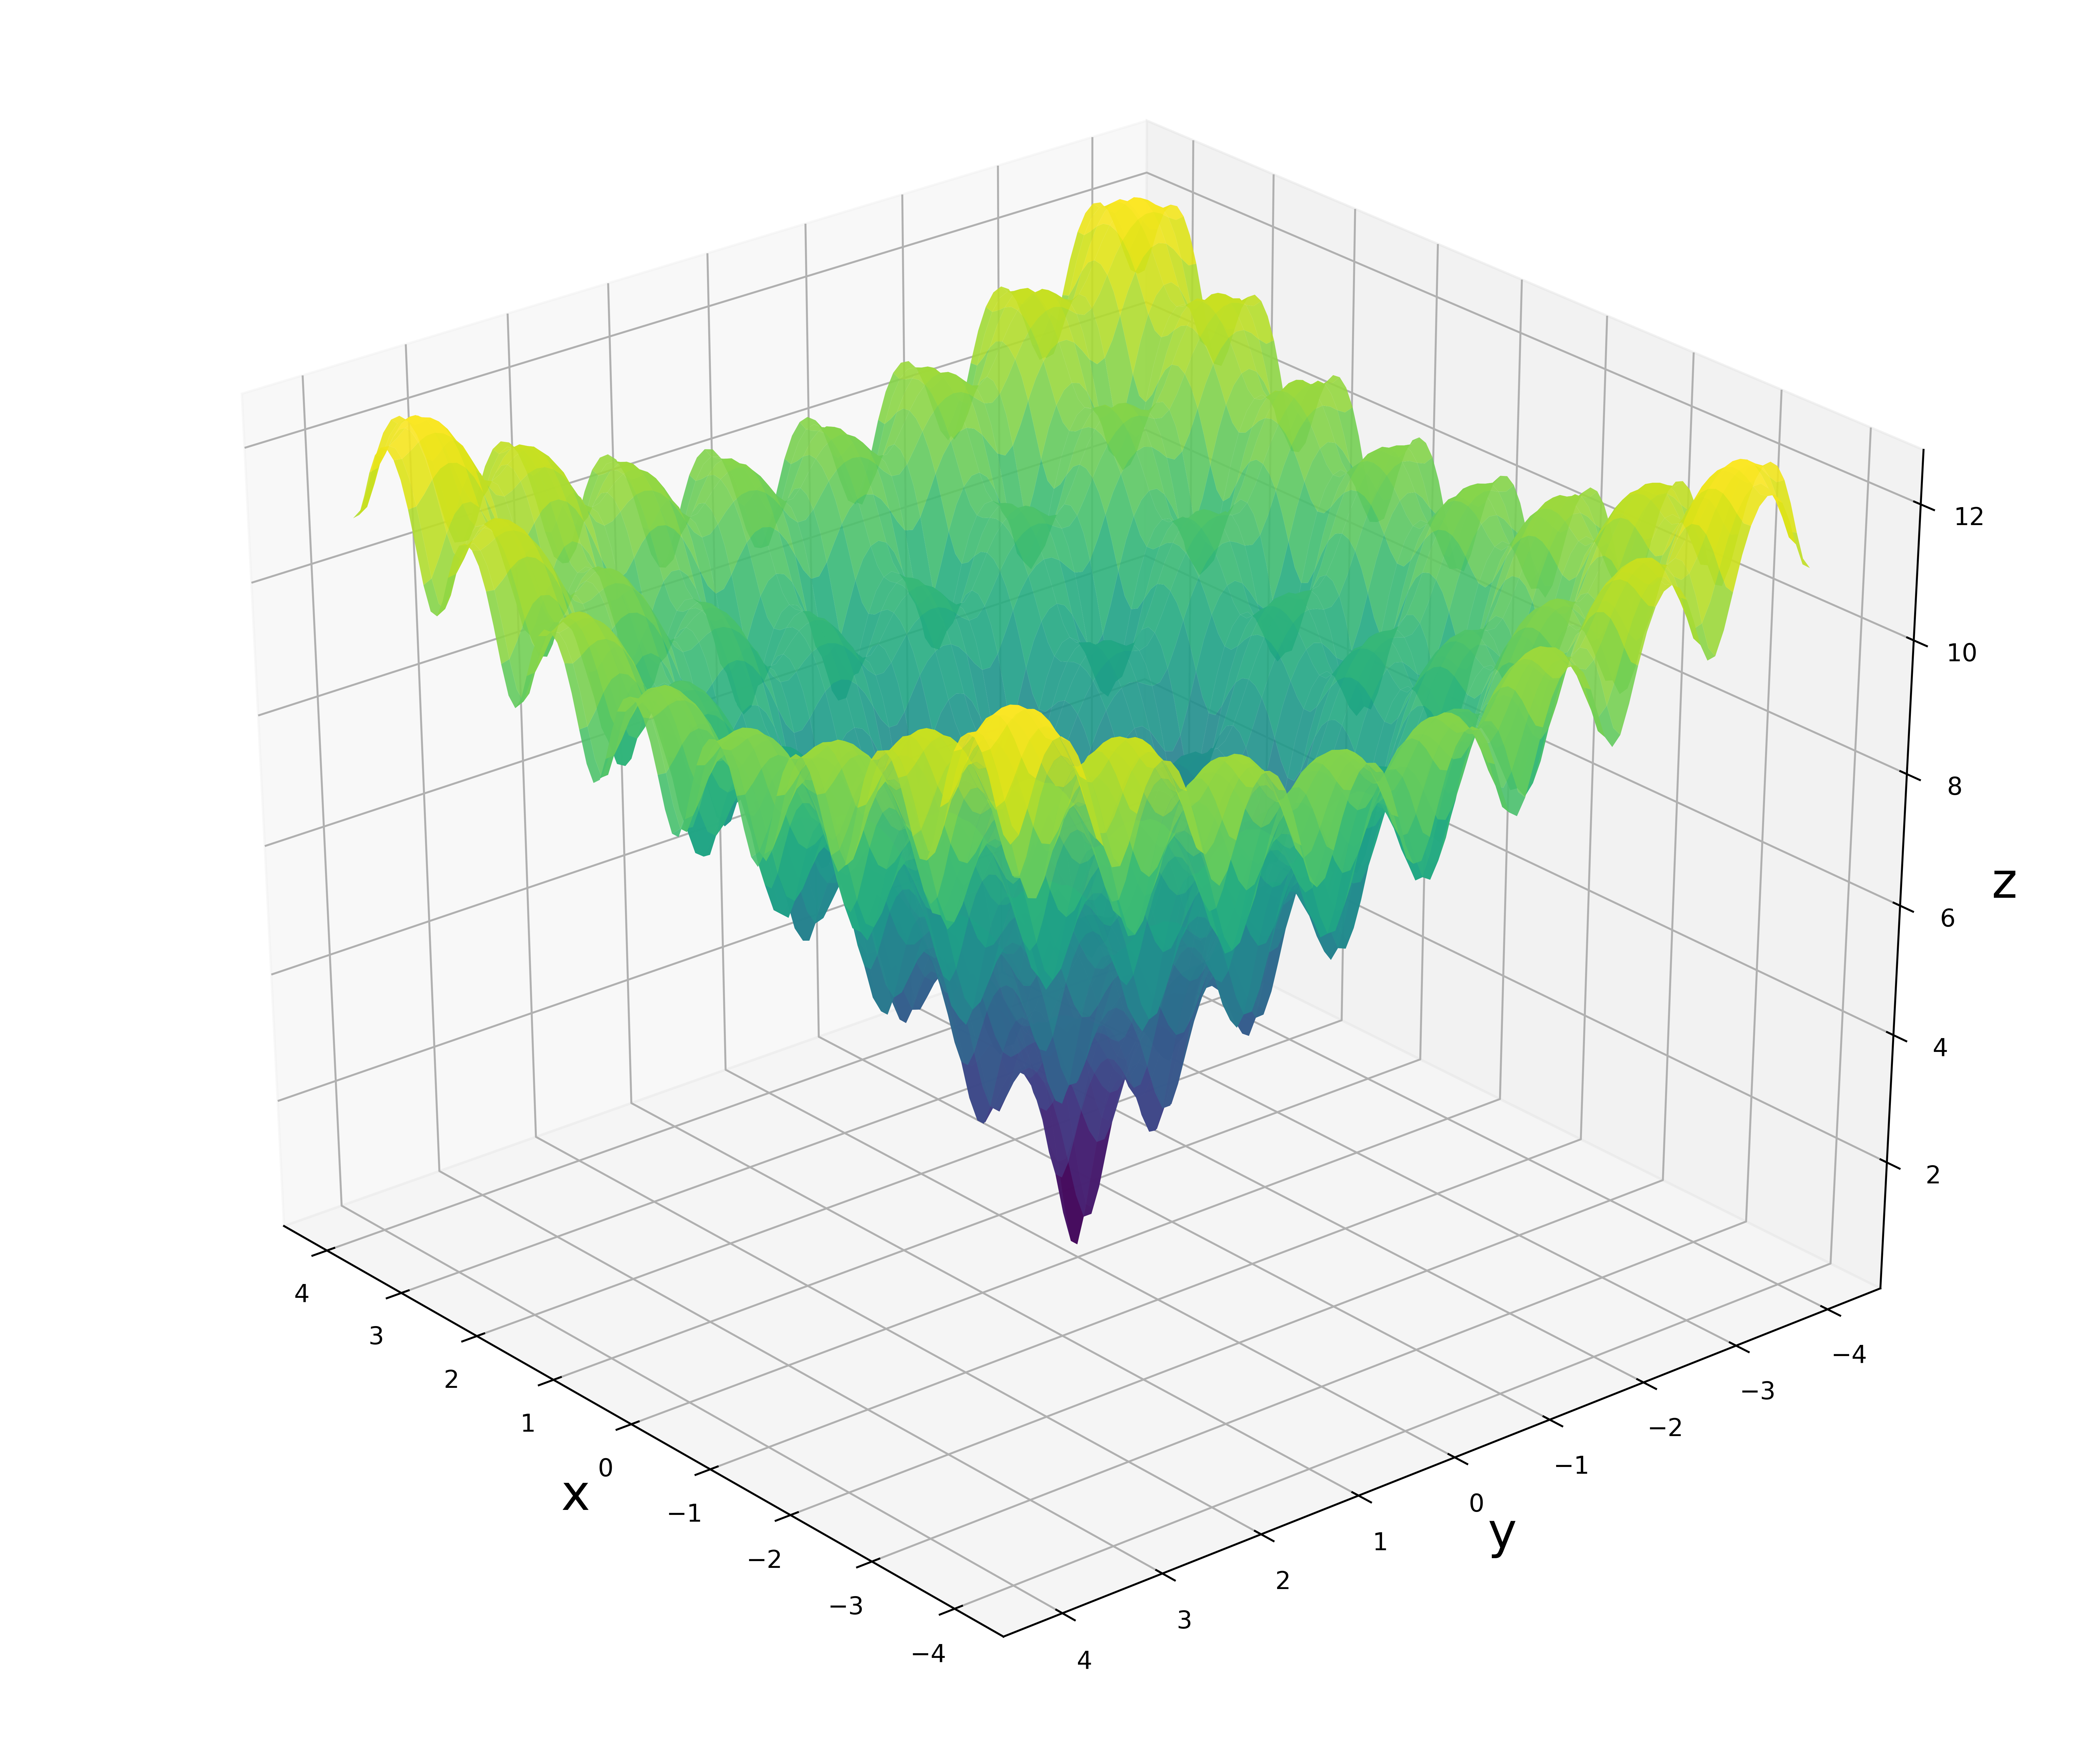
\includegraphics[width=120mm]{ackley_func}
	\caption{ --- Функция Экли в трехмерном пространстве.}
	\label{img:ackley_func}
\end{figure}


Сначала создадим класс Individual, который моделирует каждую особь в нашей популяции: присваевает каждой особи хромосому, ее длину, гены, а также значение целевой функции в точке, использующей хромосому данной особи, значение приспособленности особи. Также определим названия для каждой особи в популяции для облегчения восприятия данного класса.
\begin{pyin}
class Individual:
  def __init__(self, search_space, chromosome_len):
    self.search_space = search_space
    self.chromosome_len = chromosome_len
    self.chromosome = np.array([self.create_gene(j)
                                for j in range(chromosome_len)])
    self.target_value = None # значение целевой функции при
    # использовании данной особи
    self.fitness = None # значение приспособленности особи
    # относительно других
\end{pyin}
\begin{pyprint}
    self.name = '#' + ''.join(map(str,
                                  np.random.randint(0,9,7).tolist()))

  def create_gene(self, pos):
    return np.random.uniform(self.search_space[pos][0],
                             self.search_space[pos][1])

\end{pyprint}
\vspace{-10pt}
\begin{pyprint}
  def __repr__(self):
	  chr = '; '.join(list(map(str,
                    self.fittest_indivdual.chromosome.tolist())))
    tar = self.target_value
    return f'{self.name}: chromosome = {(chr)}; target_value = {tar}'
\end{pyprint}

Далее определим генетический алгоритм под классом GeneticAlgorithm. Гиперпараметрами нашего метода являются: количество особей в популяции (ell), количество отбираемых особей для скрещивания (k), максимальная мутация гена (mutation\_rate) и критерий останова в качестве превышения заданного количества поколений (max\_iter).
\begin{pyin}
class GeneticAlgorithm:
  def __init__(self, ell=1000, k=200, mutation_rate=0.1,
	             max_iter=100):
    """
    PARAMETERS:
    ell --- количество особей в поколении
    k --- количество особей для размножения
    mutation_rate --- максимальная мутация гена
    max_iter --- максимальное количество новых поколений
    """
    self.ell = ell
    self.k = k
    self.mutation_rate = mutation_rate
    self.max_iter = max_iter

    self.search_space = None
    self.chromosome_len = None # длина хромосомы особи
    self.best_individuals = None # k наиболее
    # приспособленных особей
    self.fittest_indivdual = None # самая приспособленная особь
    self.population = None

  def search_global(self, search_space, func):
	    """
	    INPUT:
	    search_space --- область поиска оптимума. Задается как список
	    из кортежей, где кортеж --- это область значений одного
	    аргумента функции
	    """
	    self.search_space = np.array(search_space)
	    self.chromosome_len = len(self.search_space)
	    self.best_target_value_history = []

\end{pyin}

\begin{pyprint}
    # создаем первое поколение
    self.population = self.create_population(self.search_space)

    # проходим этапы эволюции
    for i in tqdm(range(self.max_iter)):
       # оцениваем приспособленность наших особей
       self.evaluate_population(func)
       # отбираем k наиболее наиболее приспособленных особей
       self.selection()

       # формируем новые поколения
       # скрещиваем особи
       for idx in range(self.k, self.ell):
          # случайно выбираем одну из наилучших особей
          agent = np.random.choice(self.best_individuals)
          select_fitted_individual = agent
          # создаем потомка и заменяем им старую особь
          offspring = self.crossover(select_fitted_individual,
                                     self.population[idx])
          self.population[idx].chromosome = offspring

       # мутируем все особи, кроме самой приспособленной
       for individual in self.population[1:]:
          self.mutate(individual)

    return self.fittest_indivdual

  def create_population(self, search_space):
    """
    INPUT:
    search_space --- область поиска оптимума. Задается как список
    из кортежей, где кортеж --- это область значений одного
    аргумента функции
    """
		self.search_space = np.array(search_space)
    self.chromosome_len = len(self.search_space)

    return np.array([Individual(self.search_space, self.chromosome_len)
                    for i in range(self.ell)])

  def evaluate_population(self, func):
    """
    INPUT:
    func --- оптимизируемая функция, которая принимает список
    в качестве аргументов
    """
\end{pyprint}

\begin{pyprint}
    F = []

    for individual in self.population:
       individual.target_value = func(individual.chromosome)
       F.append(individual.target_value)

    for individual in self.population:
       individual.fitness = self.normalize(individual.target_value,
                                           min(F), max(F))

  def normalize(self, z, F_best, F_worst):
    """
    Нормализует значения целевой функции

    INPUT:
    z --- масштабируемое значение
    F_best --- лучшее значение целевой функции
    F_worst --- худшее значение целевой функции
    """
    return (z - F_worst) / (F_best - F_worst)

  def selection(self):
    """
    Оператор отобра
    """
    self.population = sorted(self.population,
                             key=lambda idividual: idividual.fitness,
                             reverse=True)
    self.best_individuals = self.population[:self.k]
    self.fittest_indivdual = self.population[0]

  def crossover(self, parent_fitted, parent_random):
    """
    Оператор скрещивания

    INPUT:
    parent_fitted --- одна из самых приспособленных особей
    parent_random --- случайная особь
    """
    return np.array([parent_random.chromosome[j]
                     if np.random.uniform(0, 1) < parent_random.fitness
                     else parent_fitted.chromosome[j]
                     for j in range(parent_fitted.chromosome_len)])
\end{pyprint}

\begin{pyprint}
  def mutate(self, individual):
    """
    Оператор мутации

    INPUT:
    individual --- особь, подвергающаяся мутации
    """
    individual_hat_chromosome = np.asarray([])

    for j in range(individual.chromosome_len):
       delta = np.random.uniform(-self.mutation_rate,
                                  self.mutation_rate)
       j_hat = individual.chromosome[j] + delta
       # на случай, если ген выйдет за пределы гиперпрямоугольника
       j_hat = min(max(j_hat, self.search_space[j][0]),
                   self.search_space[j][1])
       individual_hat_chromosome = np.append(individual_hat_chromosome,
                                             j_hat)

    individual.chromosome = individual_hat_chromosome
\end{pyprint}

\begin{figure}[h!!]
\centering
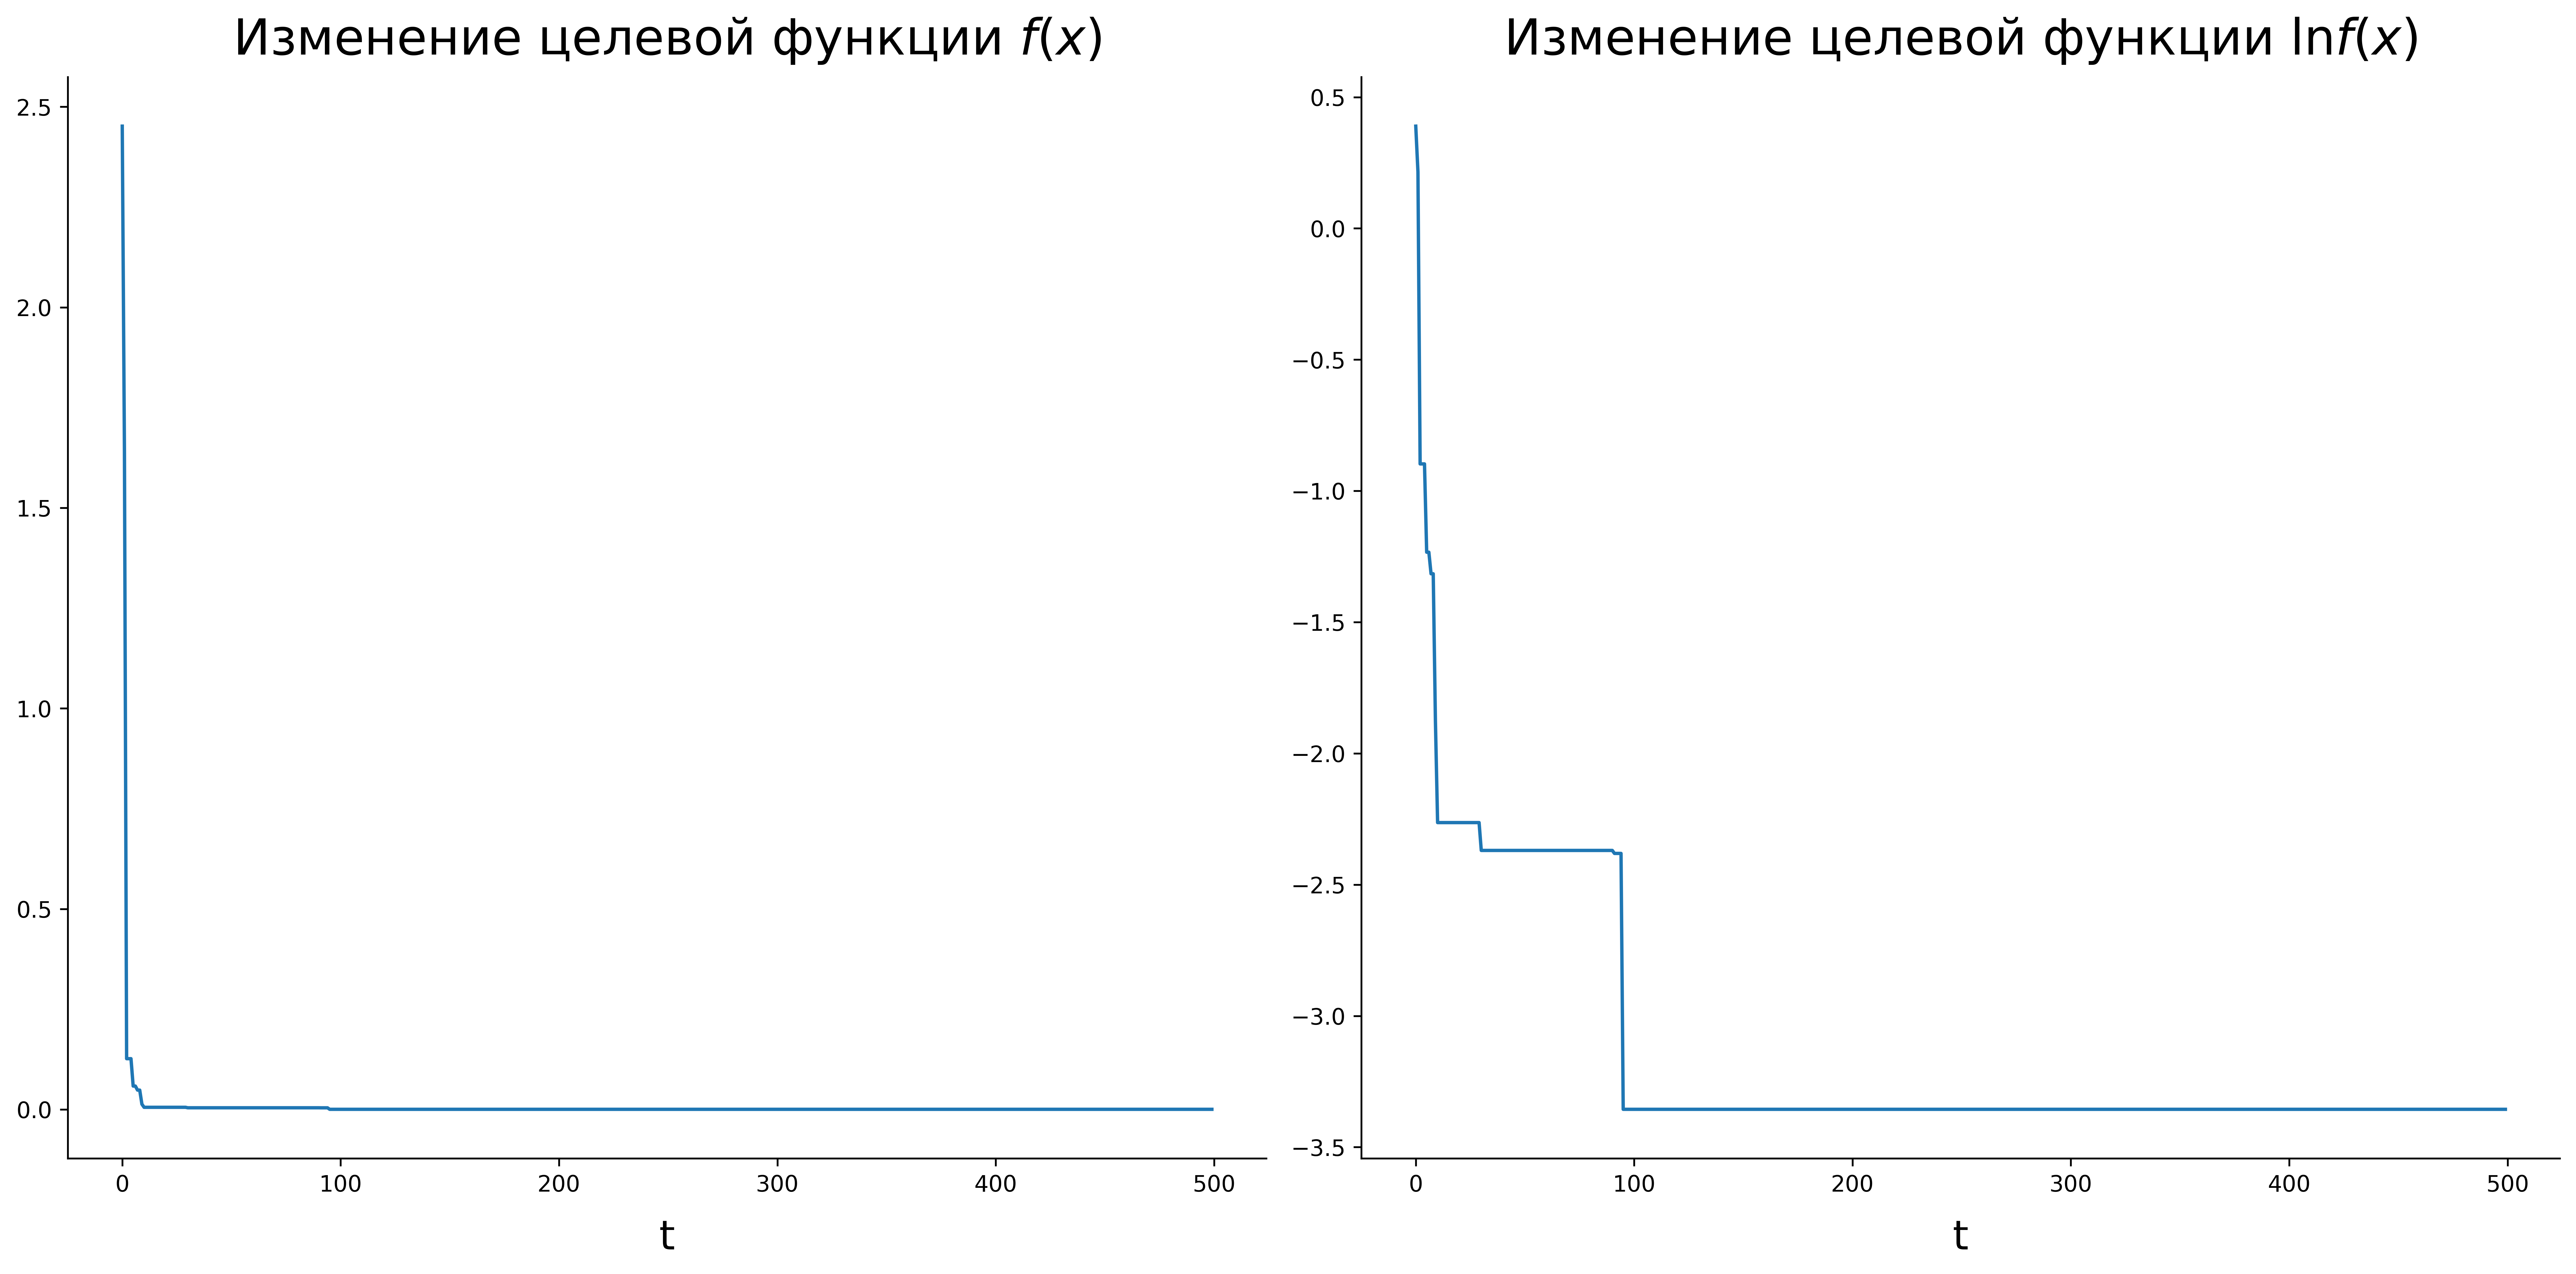
\includegraphics[width=\linewidth]{ackley_func_opt}
\caption{ --- Оптимизационный процесс.}
\label{img:ackley_func_opt}
\end{figure}

\newpage
Теперь реализуем наш алгоритм.
\begin{pyin}
np.random.seed(13)
optimizer = GeneticAlgorithm(k=200, ell=1200, mutation_rate=0.2,
                             max_iter=500)
optimizer.search_global(search_space=[(-10, 10), (-10, 10)],
                        func=ackley_func)
\end{pyin}

\begin{pyout}
#0216272: chromosome = (8.136619386361899e-05; -0.000132699205336);
target_value = 0.0004406188188861293
\end{pyout}


%%%%%%%%%%%%%%%%%%%%%%%%%%%%%%%%%%%%%%%%%%%%%%%%%%%%%%%%%%%%%%%%%%%%%%%%%%%%%%%%%%%%%%%%%%%%%%%%%%%%%%%%%%%%%%%%%%%%%%%%
%%%%%%%%%%%%%%%%%%%%%%%%%%%%%%%%%%%%%%%%%%%%%%%%%%%%%%%%%%%%%%%%%%%%%%%%%%%%%%%%%%%%%%%%%%%%%%%%%%%%%%%%%%%%%%%%%%%%%%%%


\section{Задача коммивояжера}
\noindent
Вернемся к задаче коммивояжера (TSP), расмотренной нами ранее в разделе \ref{section:TSP}. Вспомним, что метод отжига --- хоть и дал вполне приемлемый результат, --- не смог найти самый оптимальный путь. Решим данную проблему посредством генетического алгоритма. Ко всему прочему, усложним TSP: будем искать оптимальный маршрут для 52 городов.

Определим класс City, моделирующий город.


\begin{pyin}
class City:
  def __init__(self, coord, number):
    self.x = coord[0]
    self.y = coord[1]
    self.name = letters[number]

  def distance(self, city):
    return np.sqrt((self.x - city.x) ** 2 + (self.y - city.y) ** 2)
\end{pyin}

\begin{pyprint}
  def __repr__(self):
    return f'{self.name}: ({str(self.x)}; {self.y})'

part_1 = [f'{chr(i)}' for i in range(65, 65 + 26)]
part_2 = [f'{chr(i)}*' for i in range(65, 65 + 26)]
letters = part_1 + part_2
\end{pyprint}

Создадим изначальный маршрут.
\begin{pyin}
def map_city(cities_num, cities_range):
  return [City(np.random.randint(1, cities_range, size=2), j)
          for j in range(cities_num)]
\end{pyin}

\begin{pyin}
np.random.seed(13)
not_closed_road = map_city(52, 2000)
closed_road = not_closed_road + [not_closed_road[0]]
\end{pyin}

Зададим нашу целевую функцию.
\begin{pyin}
def total_distance(path, cities_lst):
  dist_lst = []
  for j in range(len(path) - 1):
     dist_lst.append(cities_lst[j].distance(cities_lst[j + 1]))
  dist_lst.append(cities_lst[j + 1].distance(cities_lst[0]))
  return sum(dist_lst)
\end{pyin}

\begin{pyin}
path = [city.name for city in closed_road]
route_dist = total_distance(path=path, cities_lst=closed_road)
\end{pyin}

\begin{figure}[h!!]
\centering
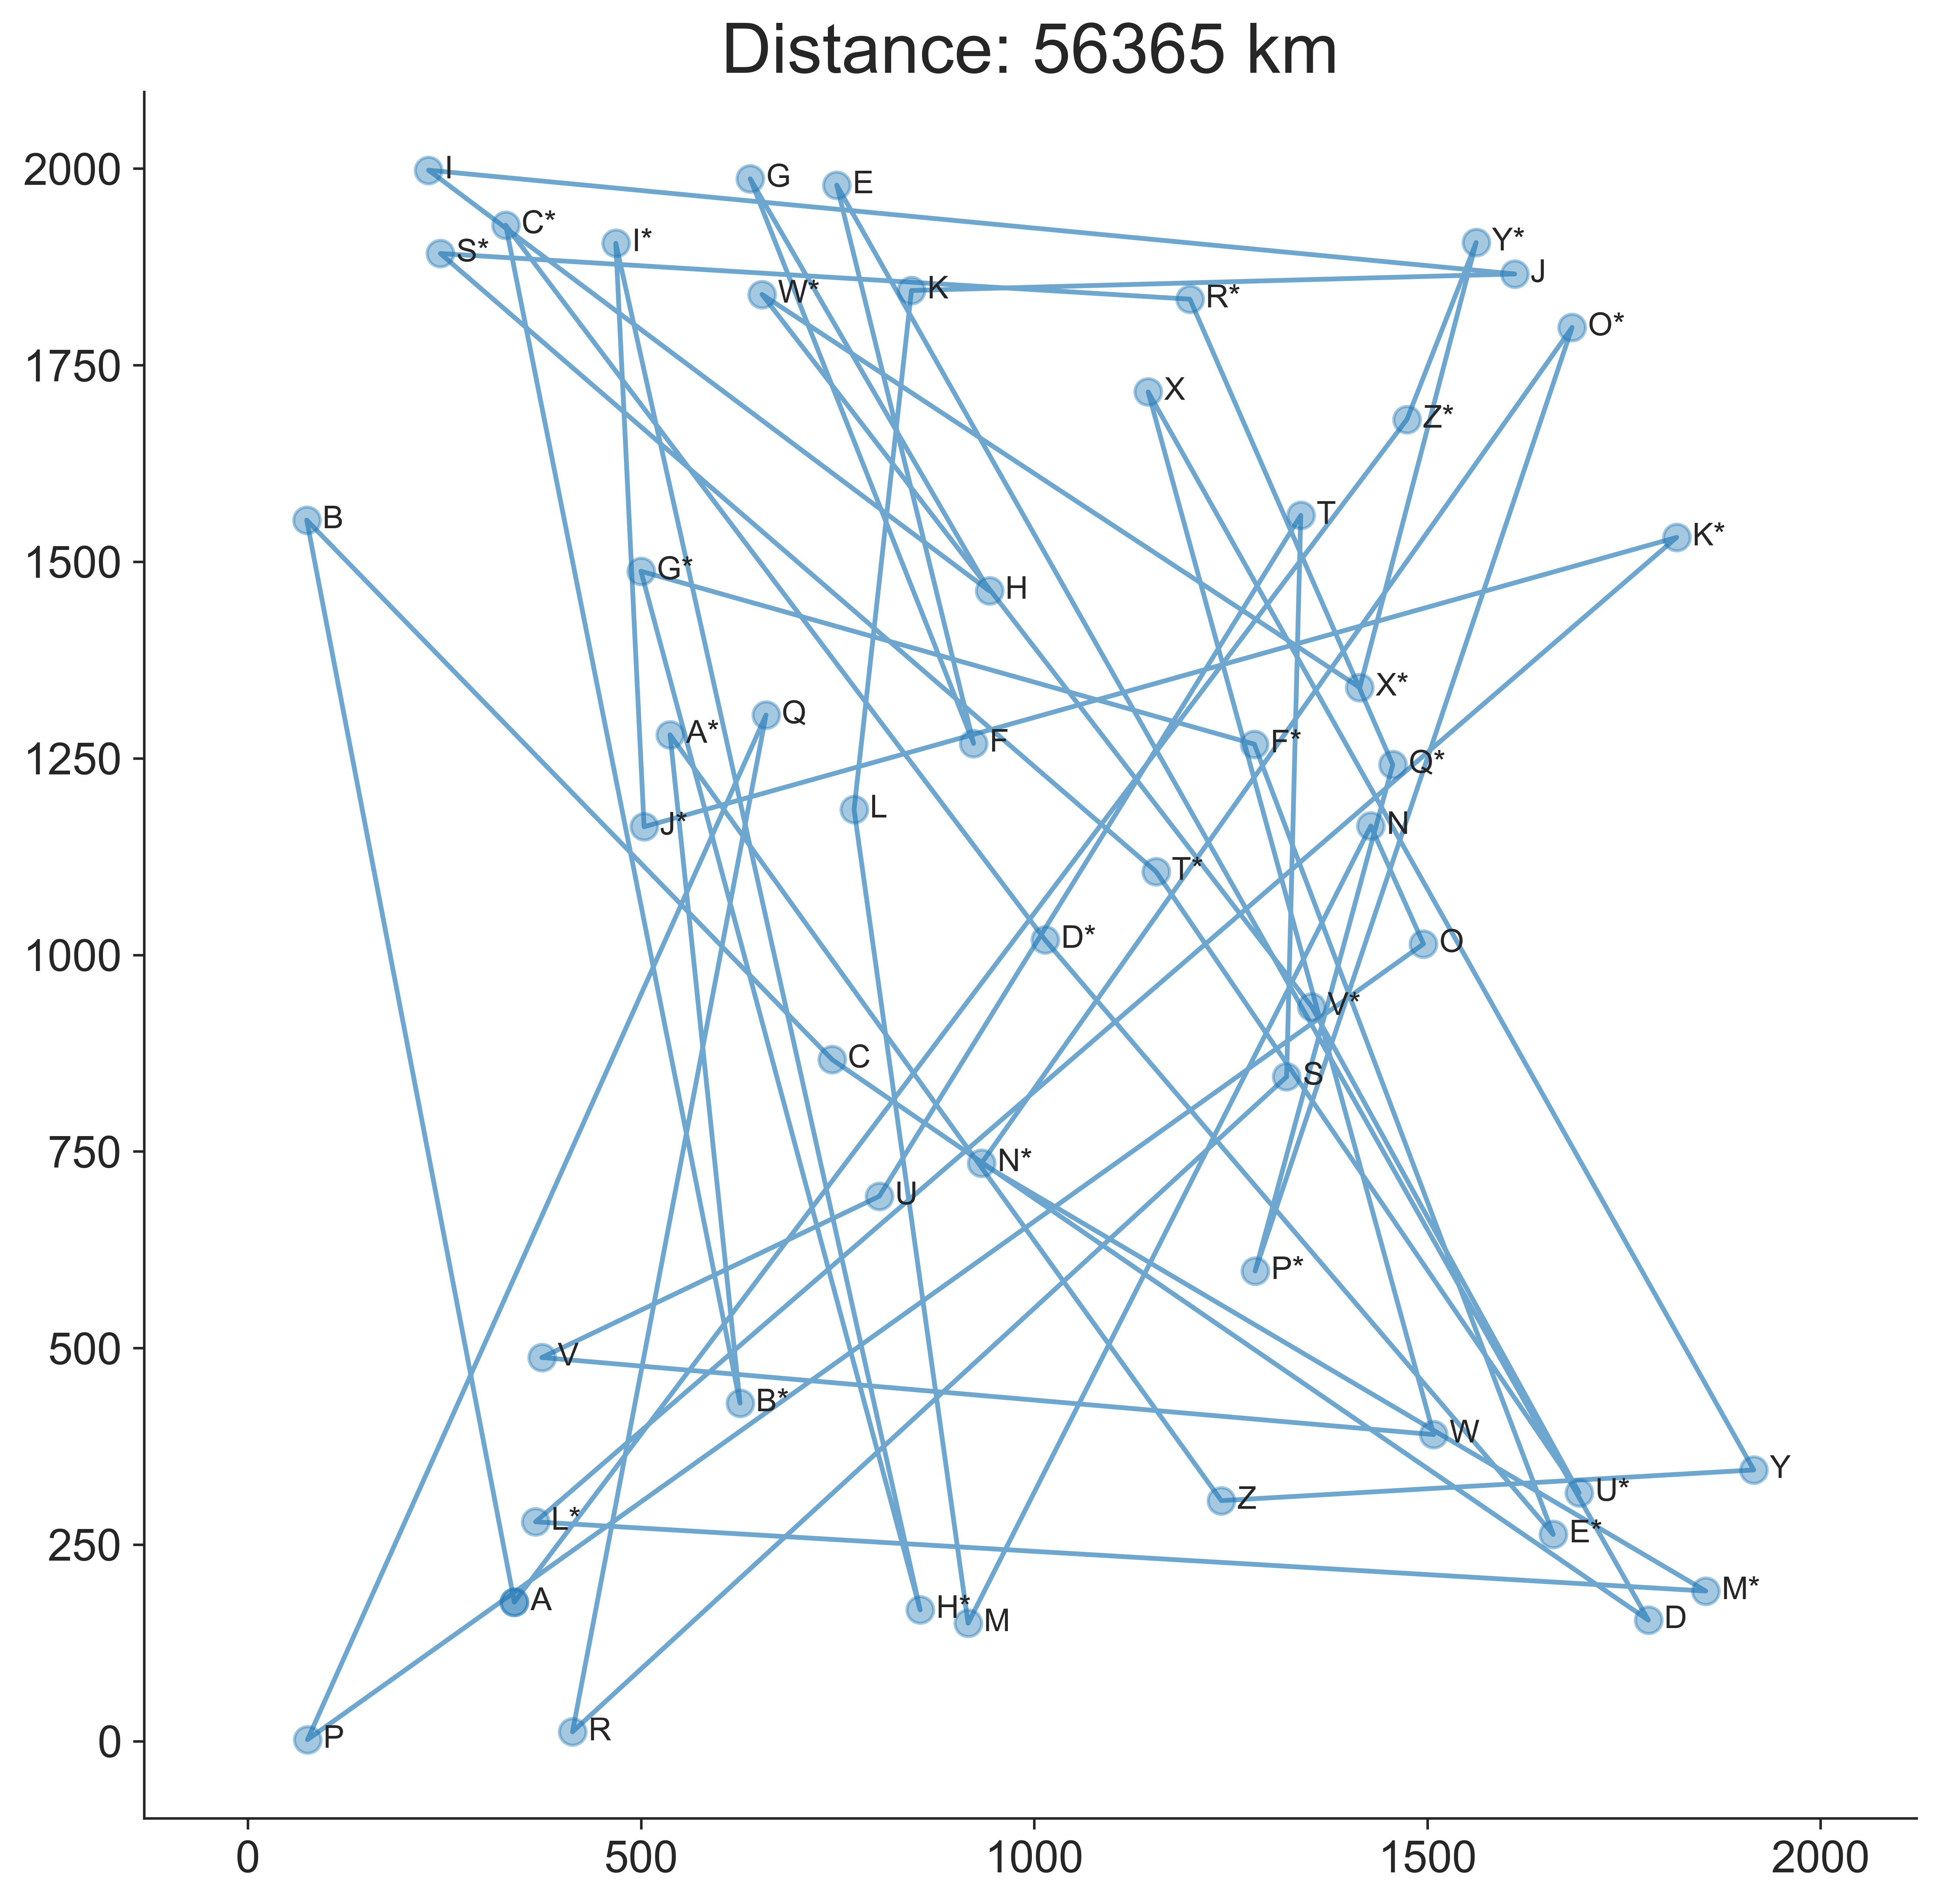
\includegraphics[width=120mm]{TSP1_}
\caption{ --- Изначальный маршрут из 52-х городов.}
\label{img:TSP1_}
\end{figure}

Определим класс Individual для моделирования особи.
\begin{pyin}
class Individual:
  def __init__(self, cities_lst, id_of_individual):
    self.map = random.sample(cities_lst[:-1],
                             len(cities_lst[:-1]))
    self.path = [city.name for city in self.map]
    self.id_of_individual = id_of_individual
    self.dist = None
    self.fitness = None
\end{pyin}

\begin{pyprint}
  def __repr__(self):
    id = self.id_of_individual
    return f'Individual {id}: Distance = {int(round(self.dist))} km'
\end{pyprint}

Теперь определим гентический алгоритм.
\begin{pyin}
class GeneticAlgorithm:
  def __init__(self, ell, k, mutation_rate, inital_map, max_iter):
    """
    PARAMETERS:
    ell --- количество особей в поколении
    k --- количество особей для размножения
    mutation_rate --- коэффициент мутации
    max_iter --- максимальное количество новых поколений
    """
    self.ell = ell
    self.k = k
    self.mutation_rate = mutation_rate
    self.inital_map = inital_map
    self.max_iter = max_iter

    self.best_individuals = None # k наиболее приспособленных особей
    self.fittest_indivdual = None # самая приспособленная особь
    self.population = None

  def search_best_path(self):
    # создаем первое поколение
    self.population = self.create_population()

    # проходим этапы эволюции
    for i in tqdm(range(self.max_iter)):
       # оцениваем приспособленность наших особей
       self.evaluate_population()
       # отбираем k наиболее наиболее приспособленных особей
       self.selection()

       # формируем новые поколения
       # скрещиваем особи
       for idx in range(self.k, self.ell):
          # случайно выбираем одну из наилучших особей
          agent = np.random.choice(self.best_individuals)
          select_fitted_individual = agent
          # создаем потомка и заменяем им старую особь
          offspring = self.crossover(select_fitted_individual,
                                     self.population[idx])
\end{pyin}

\begin{pyprint}
          self.population[idx].map = offspring
       # мутируем все особи, кроме самой приспособленной
       for individual in self.population[1:]:
          self.mutate(individual)
    return self.fittest_indivdual

  def create_population(self):
    map = self.inital_map
    return [Individual(self.map, i + 1) for i in range(self.ell)]

  def evaluate_population(self):
    F = []

    for indiv in self.population:
       indiv.dist = total_distance(indiv.path + [indiv.path[0]],
                                   indiv.map + [indiv.map[0]])
       F.append(indiv.dist)

    for indiv in self.population:
       indiv.fitness = self.normalize(indiv.dist,
                                      min(F), max(F))

  def normalize(self, z, F_best, F_worst):
    """
    INPUT:
    z --- масштабируемое значение
    F_best --- лучшее значение целевой функции
    F_worst --- худшее значение целевой функции
    """
    return (z - F_worst) / (F_best - F_worst)

  def crossover(self, parent_fitted, parent_random):
    """
    Оператор скрещивания

    INPUT:
    parent_fitted --- одна из самых приспособленных особей
    parent_random --- случайная особь
    """
    genes_1 = int(np.random.uniform(0, 1) * len(parent_fitted.path))
    genes_2 = int(np.random.uniform(0, 1) * len(parent_fitted.path))

    start = min(genes_1, genes_2)
    end = max(genes_1, genes_2)
\end{pyprint}

\begin{pyprint}
    xi = np.random.uniform(0, 1)
    if (end - start > self.ell / 2) and (xi < parent_fitted.fitness):
       child_1 = parent_fitted.map[start:end]
       child_2 = [i for i in parent_random.map if i not in child_1]
    else:
       child_1 = parent_random.map[start:end]
       child_2 = [i for o in parent_fitted.map if i not in child_1]

    return child_1 + child_2

  def mutate(self, individual):
    """
    Оператор мутации

    INPUT:
    individual --- особь, подвергающаяся мутации
    """
    for j in range(len(individual.path)):
       if np.random.uniform(0, 1) < self.mutation_rate:
          num = np.random.randint(len(individual.path))
          a, b = individual.map[j], individual.map[num]
          individual.map[num], individual.map[j] = a, b

  def selection(self):
    """
    Оператор отбора
    """
    self.population = sorted(self.population,
                             key=lambda x: x.fitness, reverse=True)
    self.best_individuals = self.population[:self.k]
    self.fittest_indivdual = self.population[0]
\end{pyprint}

Реализуем его.

\begin{pyin}
optimizer = GeneticAlgorithm(ell=1500, k=300, mutation_rate=0.001,
                             inital_map=closed_road, max_iter=1500)
optimizer.search_best_path()
\end{pyin}

\begin{pyout}
Individual 658: Distance = 11486 km
\end{pyout}

Из рисунка \ref{img:TSP2_} можно увидеть, что генетический алгоритм справился с TSP и нашел самый оптимальный маршрут.

\begin{figure}[h!!]
\centering
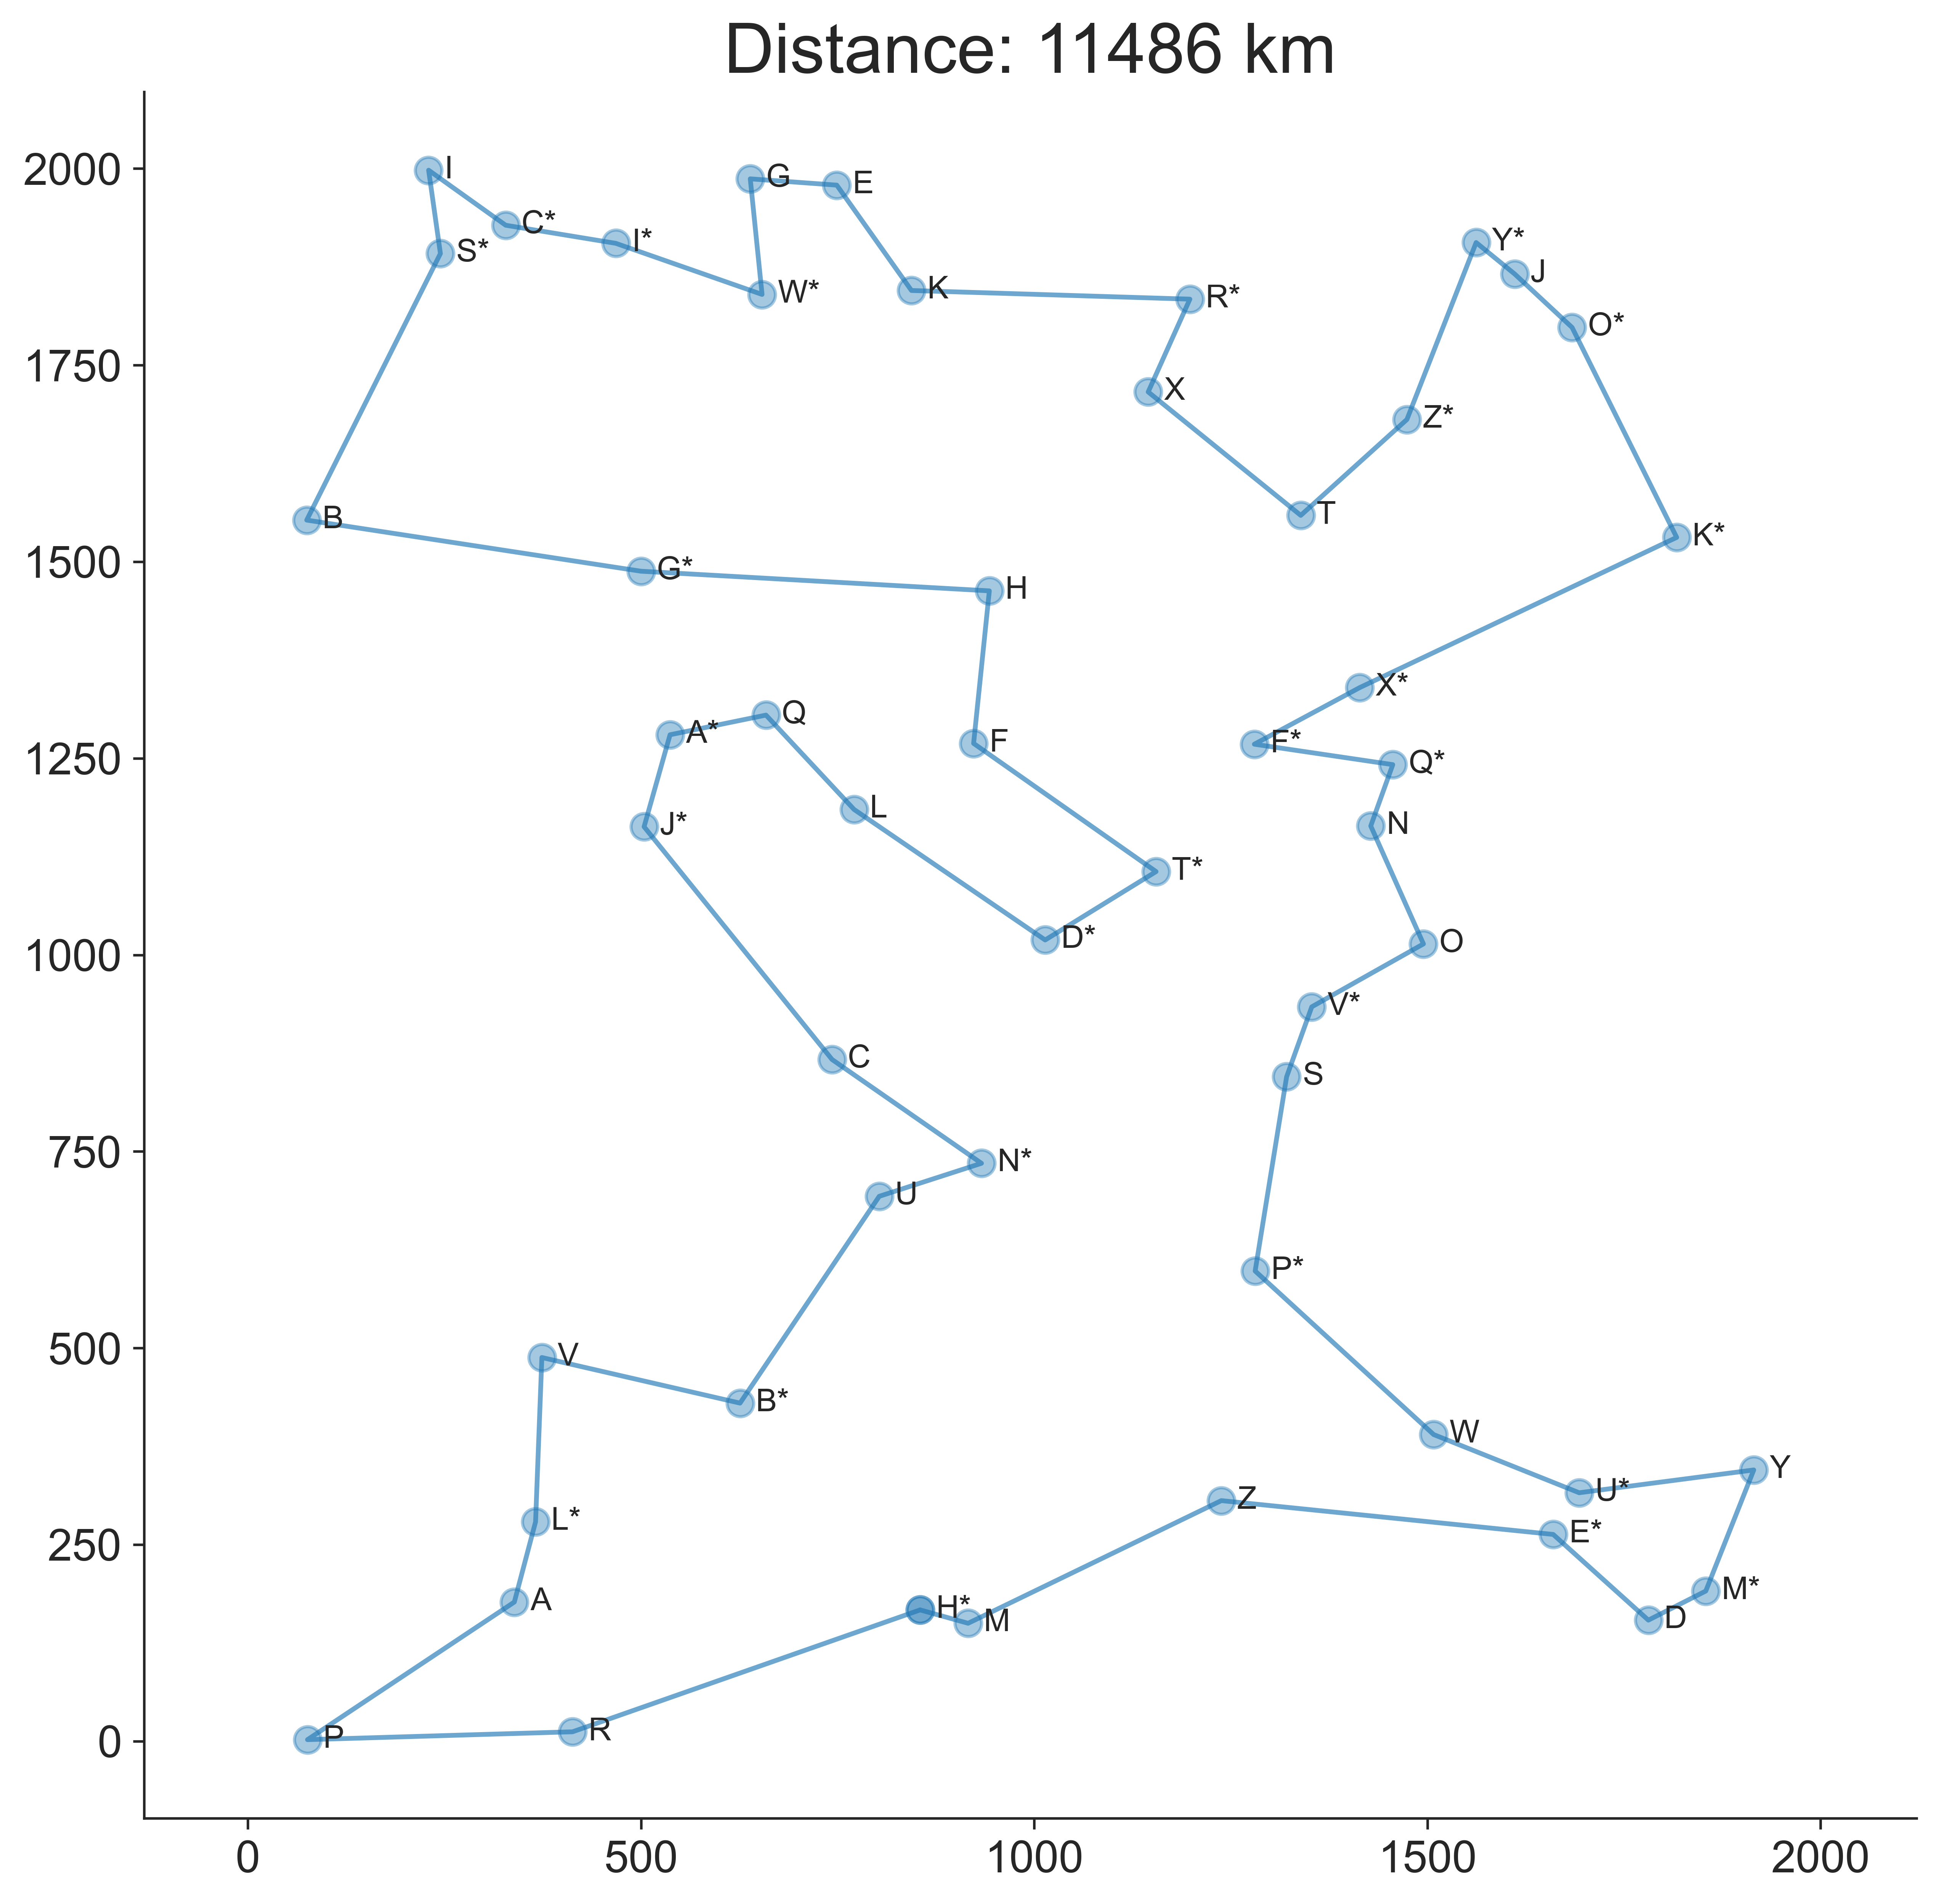
\includegraphics[width=120mm]{TSP2_}
\caption{ --- Оптимальный маршрут из 52-х городов.}
\label{img:TSP2_}
\end{figure}

\begin{figure}[h!!]
\centering
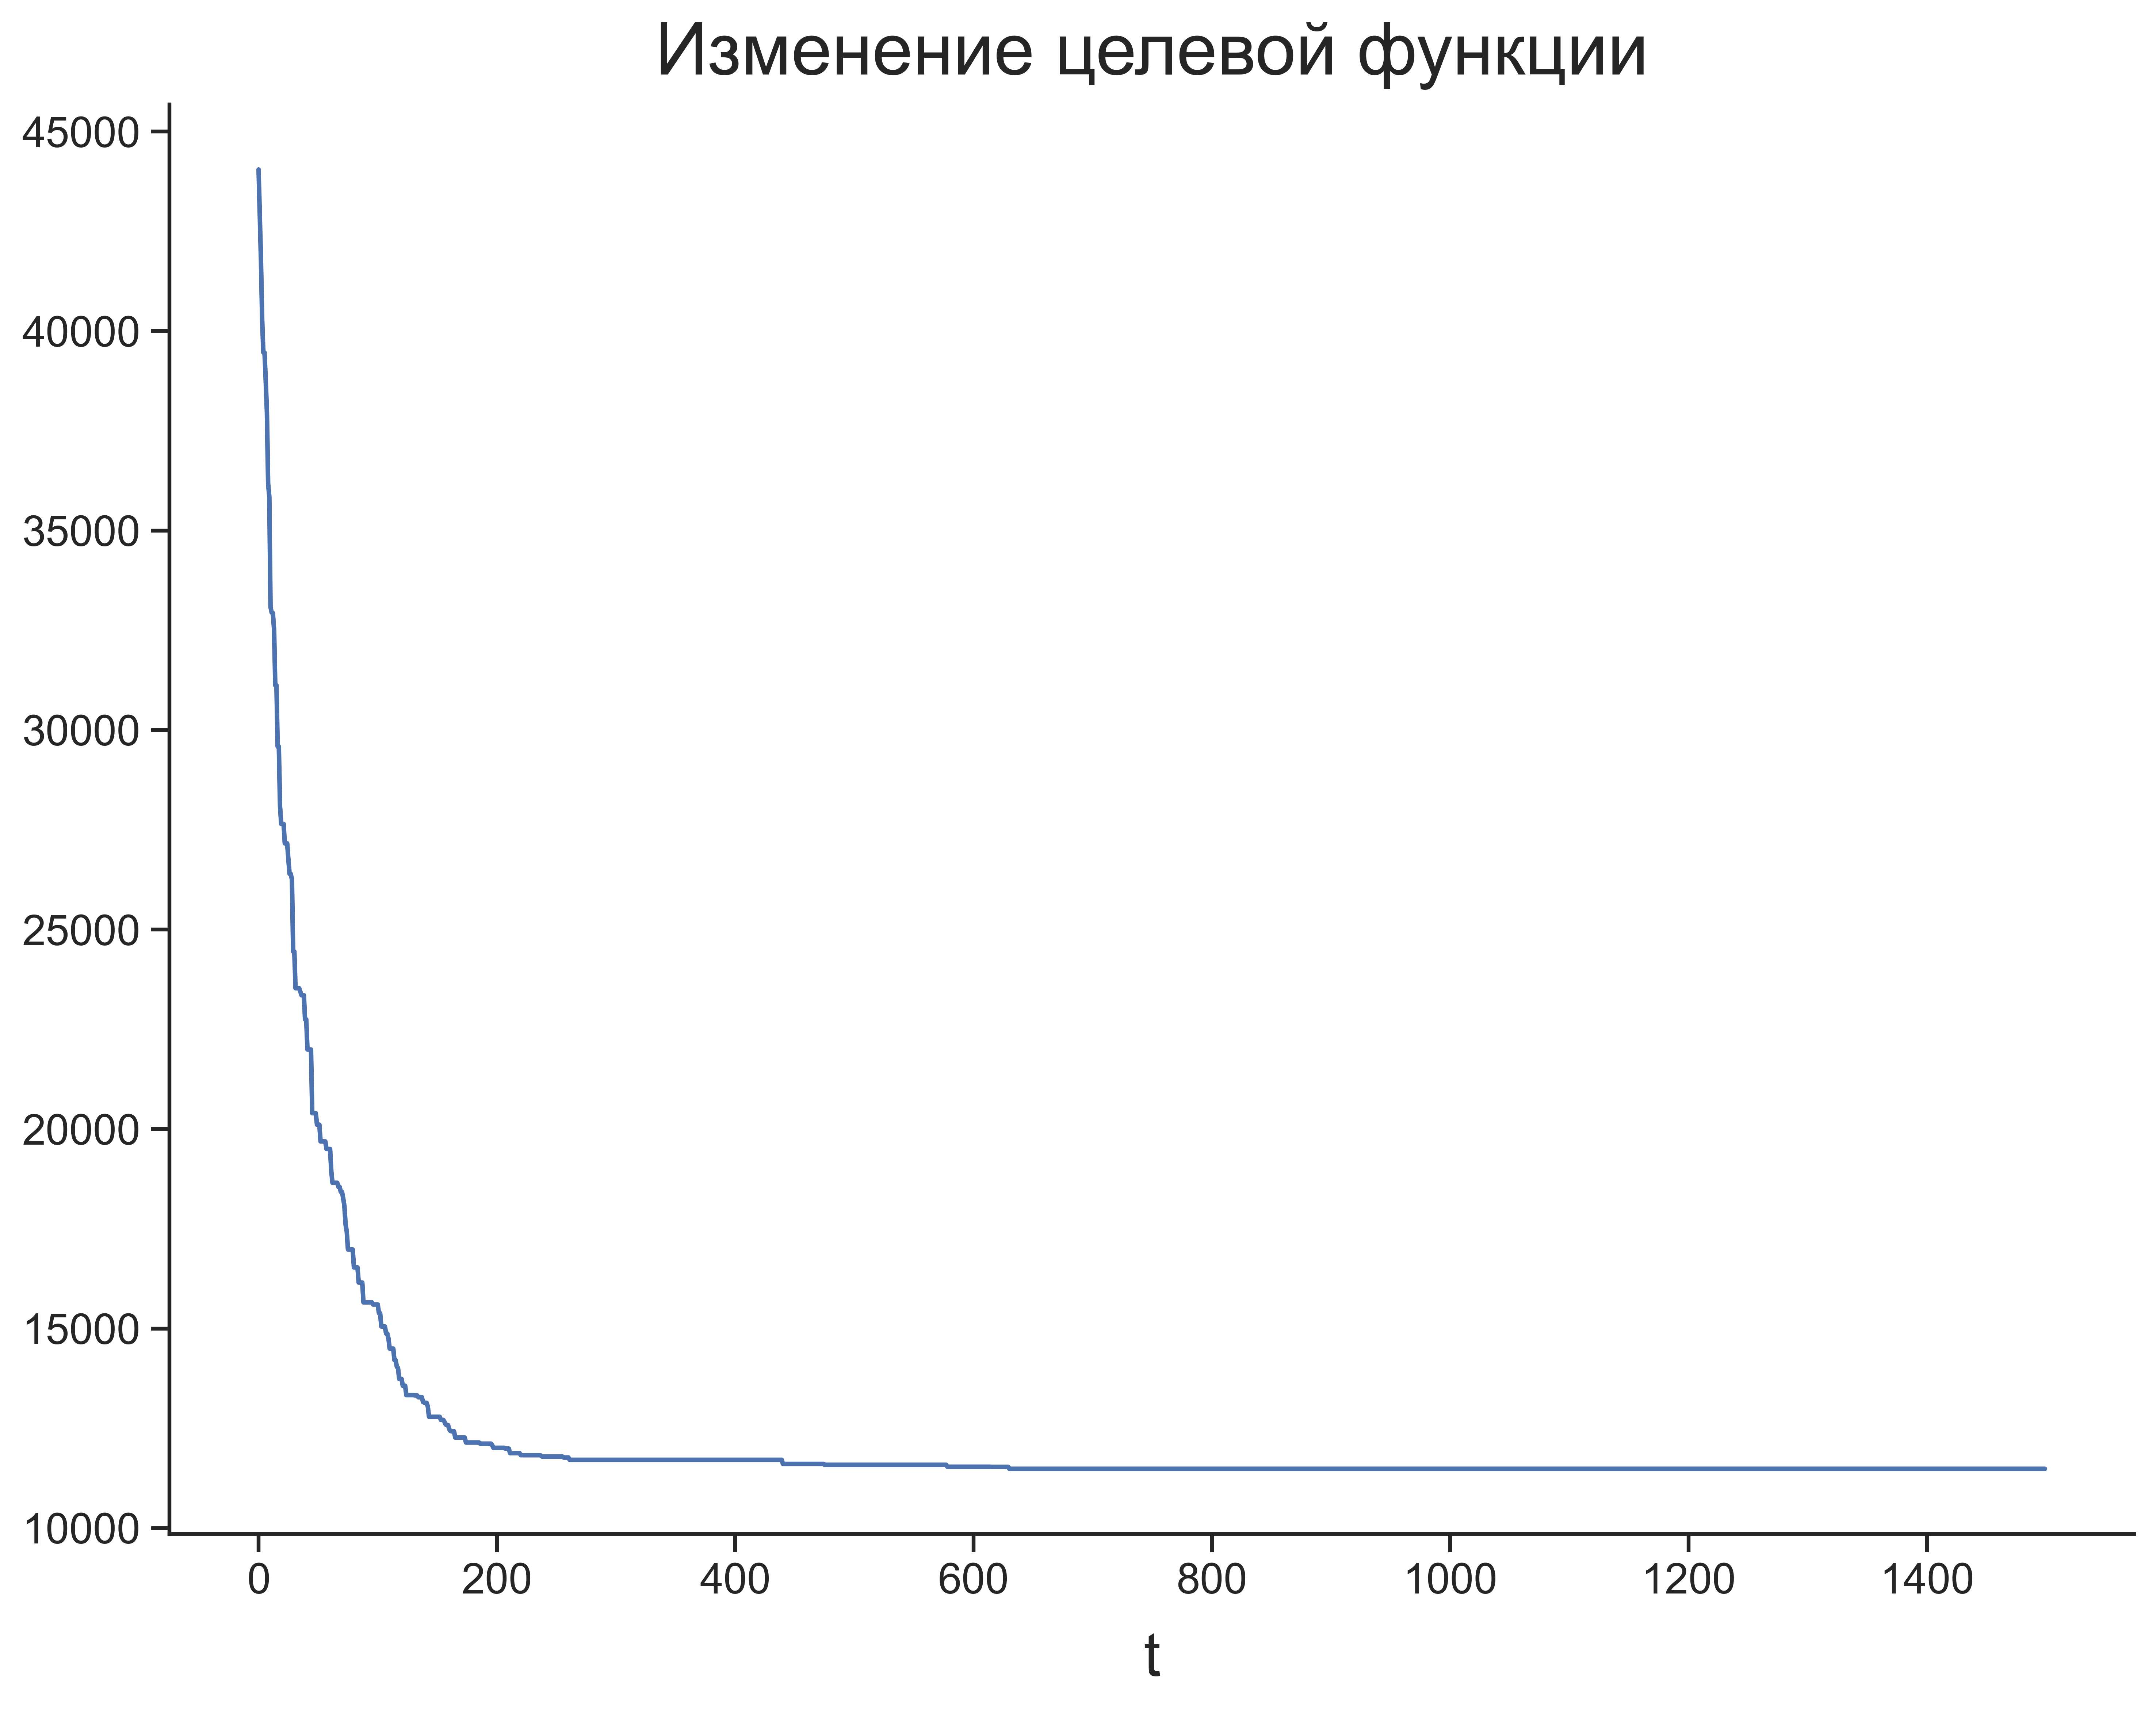
\includegraphics[width=120mm]{TSP3_}
\caption{ --- Оптимизационный процесс.}
\label{img:TSP2_}
\end{figure}


\section{Вывод}

\noindent
Рассмотрев генетический алгоритм, выявим его плюсы и минусы. РАСПИСАТЬ ЕГО МИНУСЫ ПРИМНОГО'СКТРЕМАЛЬНОСТИ И МЕДЛЕННОЙ РАБОТЕ (ПРИВЕСТИ ПРИМЕРЫ КОТОРЫЕ РАССМАТРИВАЛИ) СРАВНИТЬ С ТОЧНОСТЬЮ PSO
\noindent
\begin{table}[h!]
	\caption{Генетический алгоритм}
	\label{table:GA}
	\begin{tabular}{
	  p{\dimexpr.5\linewidth-2\tabcolsep-1.3333\arrayrulewidth}% column 1
	  p{\dimexpr.5\linewidth-2\tabcolsep-1.3333\arrayrulewidth}% column 2
	  }
	  \toprule
	  \centering Преимущества & \centering\arraybackslash Недостатки \\
		\midrule
	  1.~Не требует дифференцируемости и непрерывности исследуемой функции & 1.~Сложно найти глобальный оптимум с высокой заданной точностью  \\[.5\normalbaselineskip]
		2.~Используется для широкого класса задач & 2.~Плохо работает для многоэкстремальных функций \\[.5\normalbaselineskip]
	  3.~Не застревает в локальных минимумах, если их не много  & 3.~Достаточно медленная реализация \\[.5\normalbaselineskip]
		4.~Имеет простую реализацию & \\[.5\normalbaselineskip]
		\bottomrule
	\end{tabular}
\end{table}
